\documentclass[10pt,a4paper]{article}
\usepackage[top=1.5cm,bottom=1.4cm,left=1.7cm,right=1.7cm]{geometry}
\usepackage{booktabs,array,multirow,graphicx,amsmath,float,longtable}
\usepackage[T1]{fontenc}
\usepackage[font=footnotesize,labelfont=bf,skip=2pt]{caption}
\setlength{\parindent}{0pt}
\setlength{\parskip}{2.5pt}
\setlength{\tabcolsep}{4pt}
\newcommand{\code}[1]{\texttt{\small #1}}
\newcommand{\var}[1]{\texttt{#1}}
\pagestyle{empty}

\begin{document}
\begin{center}
{\LARGE\bfseries Optimising Attention on a CPU}\\[2pt]
{\large CS6886 Systems for Deep Learning --- Assignment 5}\\[3pt]
{\small AMD Ryzen 7 6800H (8C/16T Zen~3+), 16\,GB DDR5-4800, Windows 11.
Built with gcc 14.1.0 and \code{-O3 -march=native}.}
\end{center}
\vspace{-8pt}

\noindent\rule{\linewidth}{0.4pt}
\small
I optimised the given attention kernel step by step on my laptop. At
$N{=}4096,d{=}64$ the naive version takes 1375.9\,ms and
reaches 3.12\,GFLOP/s. My final single-threaded version
takes 47.8\,ms (89.8\,GFLOP/s), so it is
28.8$\times$ faster. With 16 threads it takes
10.6\,ms (406\,GFLOP/s),
130$\times$ faster than naive. All six variants pass \var{make check}.\par
\noindent\rule{\linewidth}{0.4pt}
\normalsize

\section{My machine}

The CPU is an AMD Ryzen 7 6800H. I read most of the specification from SMBIOS
and CPUID, and I measured the rest with small probes in \var{tools/probe.c}.
Table~\ref{tab:machine} has everything.

\begin{table}[h]
\centering\footnotesize
\caption{My machine. ``Measured'' means I ran a microbenchmark, not that I copied a datasheet.}
\label{tab:machine}
\begin{tabular}{@{}ll@{}}
\toprule
CPU & AMD Ryzen 7 6800H, Zen 3+ (family 0x19, model 0x44) \\
Cores / threads & 8 physical, 16 logical, 2 CCX $\times$ 4 cores. No P/E split. \\
Clock & 3.20\,GHz base, 4.75\,GHz rated boost. \textbf{I measured 4.29\,GHz on one core, 3.64\,GHz all-core.} \\
SIMD & AVX2 + FMA3, 256-bit, 2 FMA units per core, 16 YMM registers. No AVX-512. \\
Caches & L1D 32\,KiB/core, L2 512\,KiB/core, L3 16\,MiB (8\,MiB per CCX), 64\,B lines. \\
Memory & 16\,GB DDR5-4800 SO-DIMM, 2 channels. DRAM latency 144\,ns. \\
\bottomrule
\end{tabular}
\end{table}

Zen~3+ does two 256-bit FMAs per cycle per core. One FMA covers 8 floats and
counts as 2\,FLOP, so a core does 32 FLOP per cycle. My FMA chain gives
4.29\,GHz on one core:
\begin{equation*}
P_1 = 32\times4.29 = 134.4\ \text{GFLOP/s},\qquad
P_8 = 32\times8\times3.64 = 932\ \text{GFLOP/s}
\end{equation*}
The bandwidth I measured over a 512\,MB buffer is 25.8\,GB/s on one
thread and 36.0\,GB/s on 16 threads. DDR5-4800 dual channel is
76.8\,GB/s in theory, so I am getting about a third of it. That gives
\begin{equation*}
B_\text{theor} = 4800\times8\times2 = 76.8\ \text{GB/s},\quad
R_1 = 134.4/25.8 = 5.21\ \text{FLOP/B},\quad
R_8 = 932/36.0 = 25.87\ \text{FLOP/B}
\end{equation*}

One thing I did not expect. I ran the same clock probe in an earlier session and
got 2.38\,GHz on one core and 2.02\,GHz all-core, not 4.29\,GHz. The plan is
\emph{Best performance} and the laptop was plugged in both times, so I do not
think it is a setting. The platform seems to limit the clock depending on its
power state. So I measured the peak again before every run and I use that
session's value for all the percentages below. Otherwise the same code would
look 1.8$\times$ better or worse depending on the day.

\section{The naive kernel}

\begin{table}[h]
\centering\footnotesize
\caption{Naive kernel. Median of 5 runs after one warm-up.}
\label{tab:naive}
\begin{tabular}{@{}lrrrr@{}}
\toprule
$N/d$ & time (ms) & GFLOP/s & \% measured peak & \% rated peak \\
\midrule
1024/64 &   79.02 &  3.40 &  2.5 &  2.2 \\
2048/64 &  313.88 &  3.42 &  2.5 &  2.2 \\
4096/64 & 1375.94 &  3.12 &  2.3 &  2.1 \\
4096/128 & 3980.03 &  2.16 &  1.6 &  1.4 \\
\bottomrule
\end{tabular}
\end{table}

\textbf{Effect of $N$.} Going from 1024 to 2048 costs
4.0$\times$ and from 2048 to 4096 costs
4.4$\times$, but the work only grows by
4$\times$. The score matrix is the reason. At $N{=}2048$ it is 16\,MB and still
fits in the 16\,MB L3. At $N{=}4096$ it is 64\,MB, so every pass over it goes to
DRAM.

\textbf{Effect of $d$.} Doubling $d$ costs
2.9$\times$, not 2$\times$. In step 3 I walk
$j$ with stride $d$, so at $d{=}64$ a 64\,B line gives me four floats, and at
$d{=}128$ every load pulls a line and I use 4 bytes out of 64.

\textbf{Where the time goes.} I timed the three steps separately with
\var{tools/naive\_phases.c}. S~V is 61\,\% of
the time at 1024/64 and 76\,\% at
4096/128. I checked with \code{-fopt-info-vec} and gcc refuses to vectorise that
loop, it says \emph{``not suitable for strided load''}. So every element is a
scalar load plus one step of a 4-cycle add chain. QK$^\top$ does get vectorised
but only reaches 4.9\,GFLOP/s,
because one accumulator serialises the reduction. The softmax is only 1--4\,\%
here, so I left it alone for now.

\section{Optimisations}

\begin{table}[H]
\centering\scriptsize
\caption{All my variants, one session. Each cell: time (ms) / GFLOP/s / \% of
measured peak / speed-up over naive. Every variant passes the check, error
$1.1\times10^{-6}$ to $5.0\times10^{-6}$ against the $10^{-4}$ limit.}
\label{tab:all}
\begin{tabular}{@{}lcccc@{}}
\toprule
variant & 1024/64 & 2048/64 & 4096/64 & 4096/128 \\
\midrule
\texttt{loops} &   10.7 / 25.1 /  19 /  7.4 &   46.1 / 23.3 /  17 /  6.8 &  188.2 / 22.8 /  17 /  7.3 &  313.8 / 27.4 /  20 / 12.7 \\
\texttt{tiled} &    6.0 / 45.0 /  33 / 13.2 &   31.7 / 33.9 /  25 /  9.9 &  115.9 / 37.0 /  28 / 11.9 &  168.9 / 50.9 /  38 / 23.6 \\
\texttt{fused} &    8.2 / 32.8 /  24 /  9.6 &   34.0 / 31.6 /  24 /  9.2 &  131.4 / 32.7 /  24 / 10.5 &  295.4 / 29.1 /  22 / 13.5 \\
\texttt{best} &    3.0 / 88.7 /  66 / 26.1 &   11.5 / 93.7 /  70 / 27.4 &   47.8 / 89.8 /  67 / 28.8 &   92.3 / 93.1 /  69 / 43.1 \\
\texttt{omp} &    0.9 / 293.9 /  32 / 86.5 &    2.8 / 384.0 /  41 / 112.3 &   10.6 / 405.5 /  44 / 129.9 &   22.2 / 386.7 /  42 / 179.2 \\
\midrule
\texttt{naive} &   79.0 /  3.4 /   3 /  1.0 &  313.9 /  3.4 /   3 /  1.0 & 1375.9 /  3.1 /   2 /  1.0 & 3980.0 /  2.2 /   2 /  1.0 \\
\bottomrule
\end{tabular}
\end{table}

\textbf{(a) Loop reordering.} I transpose $K$ once, then I change the loop order
so the inner loop is an axpy instead of a dot product. An axpy has no
loop-carried dependency, so gcc vectorises it without \code{-ffast-math}:
\begin{verbatim}
S[i][:] += Q[i][k] * KT[k][:]      k outer, j inner
O[i][:] += S[i][j] * V[j][:]       j outer, k inner
\end{verbatim}
This gave 7.3$\times$. What still hurts is that
nothing is blocked, so for every row I read all of $K^{\top}$ and all of $V$ again
out of L3, about 8\,GB at $N{=}4096$. So this version is limited by L3 bandwidth,
not by the FP units.

\textbf{(b) Tiling.} QK$^\top$ now uses a $4\times16$ micro-tile. That is 8 YMM
accumulators with $k$ innermost, so per $k$ I issue 8 FMA (128\,FLOP) against two
32\,B loads and four broadcasts. 3 load cycles cover 4 FMA cycles, so the FMA
units become the limit. For S~V I block the reduction instead of the output: a
64-key slab of $V$ is 16\,KB and stays in L1 while every output row uses it, and
that keeps the $d$ accumulators in registers. Three things I had to learn by
trying:
\begin{itemize}\itemsep0pt
\item gcc will not keep the tile in registers. In plain C it vectorises the
wrong axis and spills to the stack. It only works when I write the tile with
AVX2 intrinsics.
\item A 16\,KB row is a multiple of the L1 size, so a block of rows lands on one
L1 set and thrashes. I padded every row by 64\,B and this variant went from
370.6 to 307.0\,ms at 4096/64.
\item One store per FMA caps a kernel at half of peak. My first S~V kept the
output tile in L1 and only reached 21\,\%. With the accumulators in registers it
reaches 45\,\%.
\end{itemize}
Now I get 11.9$\times$. The kernels split
22/44/34\,\%
(QK$^\top$/softmax/S~V) and QK$^\top$ runs at 71\,\% of peak.
Two problems are left. The scalar \var{expf} is
44\,\% of the kernel time, and another
14\,ms (12\,\% of the wall
time) is not in any kernel at all, it is page faults from allocating the 67\,MB
score matrix every call.

\textbf{(c) Fusion.} Row $i$ of $O$ only needs row $i$ of $S$, so I keep one
score row in a 16\,KB L1 buffer and run the three steps over it. The $N\times N$
matrix is never built. This gave 10.5$\times$,
which is slower than \var{attn\_tiled} (131 against
116\,ms) and much slower at $d{=}128$
(295 against 169\,ms).
I expected fusion to win, so I looked at the traffic. It saves about 200\,MB of
score matrix traffic but it makes every row read all of $V$, which is 4\,GB of L3
traffic at $d{=}64$ and 8\,GB at $d{=}128$. The traffic I add is bigger than the
traffic I remove.

\textbf{(d) Fastest single-threaded.} I made two changes. First I block 64
queries, so the score tile stays in cache, there is no 67\,MB allocation, and $V$
is read once per block instead of once per row. Second I replaced \var{expf} with
an AVX2 exponential: split $y=x\log_2 e$ into $n+f$ with $|f|\le0.5$, evaluate
$2^f$ with a degree-5 polynomial, and build $2^n$ by writing $n+127$ into the
exponent field. It is 8.5$\times$ faster than libm (16.8\,M calls: 5.0\,ms
instead of 42.3\,ms), and the whole kernel still stays within
$5.0\times10^{-6}$ of the naive result. Now I get 28.8$\times$ and
89.8\,GFLOP/s, which is 67\,\% of
the measured peak. That is 2.4$\times$ faster
than \var{tiled} and 2.7$\times$ faster than
\var{fused}.

\section{OpenMP}

I parallelised the query blocks. $K^{\top}$ is built once before the parallel
region starts. I do not need a barrier inside it: the blocks write disjoint
$64\times d$ slices of $O$, everything they read is shared and read-only, and the
slices are 16\,KB apart so there is no false sharing. One surprise here. With
\code{OMP\_PROC\_BIND=close} Windows puts both threads of a 2-thread run on the
two SMT siblings of one core, and I measured 53.9\,ms instead of 45.3\,ms. So the
numbers in Table~\ref{tab:omp} are without binding.

\begin{table}[H]
\centering\footnotesize
\caption{Strong scaling. Speed-up is against the same binary at one thread.}
\label{tab:omp}
\begin{tabular}{@{}llrrrr@{}}
\toprule
$N/d$ & threads & time (ms) & speed-up & eff.\ (\%) & GFLOP/s \\
\midrule
\multirow{5}{*}{4096/64} &  1 &    50.37 &  1.00 &  100 &   85.3 \\
 &  2 &    25.29 &  1.99 &  100 &  169.8 \\
 &  4 &    13.59 &  3.71 &   93 &  316.1 \\
 &  8 &    10.83 &  4.65 &   58 &  396.5 \\
 & 16 &    10.59 &  4.76 &   30 &  405.5 \\
\midrule
\multirow{5}{*}{4096/128} &  1 &    91.82 &  1.00 &  100 &   93.6 \\
 &  2 &    49.30 &  1.86 &   93 &  174.2 \\
 &  4 &    27.13 &  3.38 &   85 &  316.6 \\
 &  8 &    24.90 &  3.69 &   46 &  345.0 \\
 & 16 &    22.21 &  4.13 &   26 &  386.7 \\
\bottomrule
\end{tabular}
\end{table}

Up to 4 threads it is close to linear. 8 threads give
4.65$\times$, which is
58\,\% efficiency, and I think the
clock explains the gap: all-core is 3.64\,GHz against 4.29\,GHz on one core, so the
best I can get here is $8\times(3.64/4.29)={8*3.64/4.29:.1f}\times$. 16 threads give
4.76$\times$. The kernel is FMA bound and
the two SMT threads of a core share the same two FMA pipes. The whole machine
reaches 932\,GFLOP/s at 16 threads against
$8\times134.4=1075$ from the single core peak, so SMT adds about a
quarter and not double. Efficiency is counted against thread count, so it drops
fast even though the time still improves.

\section{Roofline}

I used the numbers I measured in section 1: 134.4\,GFLOP/s at
25.8\,GB/s on one core. Intensity is the useful FLOPs divided by the
bytes a variant has to move. The numerator is always $4N^2d$; I did not count the
softmax in the FLOPs. For the bytes I counted what each kernel actually needs:
\begin{equation*}
(4Nd+3N^2)\times4 = 205.5\ \text{MB}\Rightarrow 20.9,\qquad
4Nd\times4 = 4.19\ \text{MB}\Rightarrow 1024,\qquad
(4Nd+Nd+\tfrac{N}{64}Nd)\times4 \Rightarrow 59.4
\end{equation*}
which are (naive, loops, tiled), (fused) and (best, omp) in that order.

\begin{table}[H]
\centering\footnotesize
\caption{Every variant at $N{=}4096,d{=}64$ against the roofline.}
\label{tab:roof}
\begin{tabular}{@{}lrrrr@{}}
\toprule
variant & AI (FLOP/B) & ms & GFLOP/s & \% of relevant peak \\
\midrule
\texttt{naive} &   20.9 & 1375.94 &    3.1 &    2 \\
\texttt{loops} &   20.9 &  188.19 &   22.8 &   17 \\
\texttt{tiled} &   20.9 &  115.95 &   37.0 &   28 \\
\texttt{fused} & 1024.0 &  131.42 &   32.7 &   24 \\
\texttt{best} &   59.4 &   47.84 &   89.8 &   67 \\
\texttt{omp} &   59.4 &   10.59 &  405.5 &   44 \\
\bottomrule
\end{tabular}
\end{table}

\begin{figure}[H]
\centering
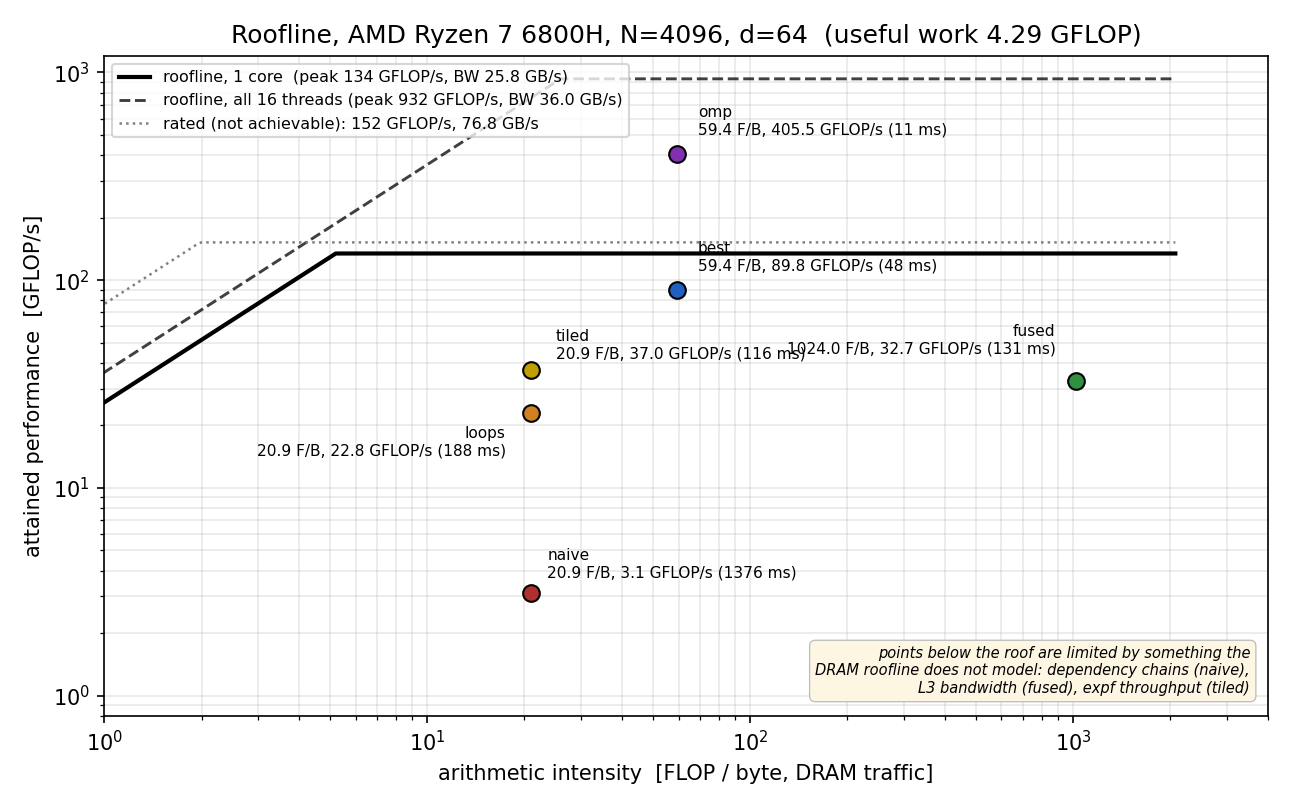
\includegraphics[width=0.84\linewidth]{plots/roofline.png}
\caption{My roofline at $N{=}4096,d{=}64$.}
\label{fig:roof}
\end{figure}

\textbf{What limits each one.} \var{naive} is to the right of the ridge, so the
roofline says it should reach 134.4\,GFLOP/s, and I get
2.3\,\%. The roofline cannot explain that, because the strided loop
costs one dependent add per element. \var{loops} is compute bound by the model and
5.9$\times$ below it, and its real limit is L3
bandwidth. \var{tiled} has QK$^\top$ at 71\,\% of peak, so what
holds it back is \var{expf} and the page faults. \var{fused} is
197$\times$ past the ridge by the
DRAM model and I only get 24\,\%, because its
limit is L3 bandwidth, which is above DRAM and does not show on this plot.
\var{best} reaches 67\,\% of peak and what is left is the softmax,
S~V at 45\,\% of peak, and reading $V$ again. \var{omp} sits above
the single-core roofline, which makes sense because it uses all the cores, and
against the all-core roof it reaches 44\,\%.

\section*{How I did all this}

The handout \var{Makefile} is unchanged. My laptop has no \var{make} (the MSYS2
one cannot start its signal pipe here) and no \var{clang}, so I ran everything
through \var{tools/bench.py}, which does the same steps with gcc 14.1.0 and runs
the same check rule. \code{-march=native} picks \var{znver3}, the same ISA the
Makefile would pick with clang. Every number is the median of 5 runs after one
warm-up. I kept all the tables in one session because the clock moves between
sessions. I only used \var{libm}, \var{immintrin.h} and \var{omp.h}, no BLAS or
other math library. The driver in each file is untouched from
\var{attn\_naive.c}. \var{results.csv} has 40 rows, including every thread count.

\section*{Checking it against the handout}

{\footnotesize
\begin{longtable}{@{}>{\raggedright\arraybackslash}p{6.0cm}
                    >{\raggedright\arraybackslash}p{7.6cm}l@{}}
\caption{What the handout asked for and where I did it.}
\label{tab:audit}\\
\toprule
Requirement & What I did & Where \\
\midrule
\endfirsthead
\toprule
Requirement & What I did & Where \\
\midrule
\endhead
\bottomrule
\endfoot
\var{machine\_spec.txt}: all fields, cores incl.\ P/E, clocks, SIMD, caches,
memory size and type & Filled everything from SMBIOS and CPUID, then measured
the parts I could. P/E is none, the design is homogeneous. & Table~\ref{tab:machine} \\
\addlinespace
Q1: peak FP32 for one and all cores, bandwidth, ridge point, with calculations &
Showed the arithmetic for $P_1$, $P_8$, $B$ and both ridges. & \S1 \\
\addlinespace
Q2: time, GFLOP/s, \% of peak per input; effect of $N$ and $d$; where the time
goes & Table~\ref{tab:naive} has both peak columns, then I wrote two paragraphs
on $N$ and $d$ and timed the three steps. & \S2 \\
\addlinespace
Q3: the same measurements as Q2 plus speed-up; \var{make check} passes; what
limits each variant & Table~\ref{tab:all} gives time, GFLOP/s, \% of peak and
speed-up for every input. All six pass. Every variant has a limit sentence. &
  \S3 \\
\addlinespace
Q3(a--d): reorder loops, cache and register tiling, fuse so $N\times N$ is never
stored, maximum single-threaded & Axpy interchange, then a $4\times16$ YMM tile,
then one score row in L1 with no $N^2$ allocation, then query blocking plus an
AVX2 exp. & \S3(a)--(d) \\
\addlinespace
``No BLAS or other math libraries'' & I only included \var{libm},
\var{immintrin.h} and \var{omp.h}. & last section \\
\addlinespace
Q4: OpenMP, several thread counts, time, speed-up, efficiency, scaling
explained & Ran 1, 2, 4, 8 and 16 threads, then explained the clock and SMT
limits. & Table~\ref{tab:omp} \\
\addlinespace
Q5: roofline from Q1 numbers, every variant at $N{=}4096,d{=}64$, intensity
computation, limiting factor & Table~\ref{tab:roof} and Figure~\ref{fig:roof},
with the byte counts and one limit per variant. & \S5 \\
\addlinespace
Submission structure; \var{results.csv} rows for each thread count &
Kept the structure exactly. \var{results.csv} has 40 rows. & repository \\
\end{longtable}
}

\end{document}
